\documentclass[a4paper]{jacow}
\usepackage{mathtools}
\usepackage{amsmath}
\usepackage{xfrac}
\usepackage{xparse}
\usepackage{subcaption}
\usepackage{graphicx}
\usepackage{url}
\usepackage{paralist}
\usepackage{multirow}

\let\oldvec\vec
\renewcommand{\vec}{\boldsymbol}
\DeclareDocumentCommand{\bkt}{sm}{\IfBooleanTF{#1}{\left[ #2 \right]}{\left(#2\right)}}
\DeclareDocumentCommand{\ddt}{m}{\frac{\mathrm{d} {#1}}{\mathrm{d} t}}
\DeclareDocumentCommand{\pddx}{mO{t}O{}}{\frac{\partial^{#3} {#1}}{\partial {#2}^{#3}}}
\newcommand{\w}{\omega}
\newcommand{\W}{\Omega}
\newcommand{\avg}[1]{\langle {#1} \rangle}
\newcommand{\nbar}{\bar n}


\begin{document}
\title{Spin Motion Perturbation Effect on the EDM Statistic in the Frequency Domain Method}
\author{A. E. Aksentyev$^1$\footnotemark[2], Institut f\"ur Kernphysik, Forschungszentrum J\"ulich, J\"ulich, Germany \\$^1$ also at National Research Nuclear University ``MEPhI,'' Moscow, Russia}
\maketitle
\footnotetext[2]{a.aksentev@fz-juelich.de}
\begin{abstract}
  The spin precession axis of a particle involved in betatron motion precesses about the invariant spin axis
  defined on the closed orbit (CO). This precession can be observed in polarization data as a rapid,
  small-amplitude oscillation on top of the major effect oscillation caused by the precession of spin
  about the CO axis. The frequency of this latter oscillation is used in the Frequency Domain methodology
  as the EDM observable. It is estimated by fitting polarimetry data by a sine function; the rapid
  oscillations, therefore, constitute a model specification error.
  This model error will introduce a bias into the frequency estimate. In the present work we investigate
  how this bias changes depending on the beam revolution direction, its stability over time, and
  the EDM estimate error introduced by it.
\end{abstract}

\section{Frequency Domain methodology}
Frequency Domain (FD)~\cite{Senichev:FDM} is a Storage Ring method of search for the
Electric Dipole Moment (EDM) of a fundamental particle.~\cite{BNL:SREDM}
It belongs to the Frozen Spin~\cite{BNL:Deuteron2008} category
of such methods, i.e., the Magnetic Dipole Moment (MDM) component of spin precession is minimized. However,
the original Frozen Spin method proposed in~\cite{BNL:Deuteron2008} is a Space Domain
method~\cite[p.~4]{Talman:ElectricRings}: the EDM is estimated from the value $P_y$ of
the vertical component of the beam polarization vector at the end of the measurement cycle. This approach has
two obvious weaknesses:
\begin{inparaenum}[\itshape a\upshape)]
\item it puts very stringent constraints on the precision of the accelerator optical elements alignment, and
\item it poses a challenging task for polarimetry.~\cite[p.~6]{Mane:SpinWheel}
\end{inparaenum}

The former is to minimize the magnitude of
the vertical plane MDM precession frequency:~\cite[p.~11]{BNL:Deuteron2008}
\begin{equation}\label{eq:BNL_syst_err}
\w_{syst} \approx \frac{\mu\avg{E_v}}{\beta c\gamma^2},
\end{equation}
induced by field imperfections. The latter is due to the requirement of detecting a change of about
$5\cdot 10^{-6}$ to the cross section $\varepsilon_{LR}$ in order to get to the EDM sensitivity level
of $10^{-29}~e\cdot cm$.~\cite[p.~18]{BNL:Deuteron2008}

EDM search methods in the Frequency Domain circumvent the above problems: the polarization vector is made to
rotate about a nearly-constant, definite direction vector $\nbar$, with a frequency that is large enough so that
the beam polarization is easily measureable at all times. This ``Spin Wheel'' may be
externally applied~\cite{Koop:SW}, or it may use the
field imperfection frequency~\eqref{eq:BNL_syst_err}~\cite{Senichev:FDM}. The latter is made possible by the fact
that $\w_{syst}$ changes sign when the beam revolution direction is reversed.~\cite[p.~11]{BNL:Deuteron2008}

The frequency of oscillation of $P_y$ is estimated via a fit of the polarimetry data to the model
\begin{equation}\label{eq:fit_model}
  f(t) = a\cdot\sin(\w\cdot t + \delta).
\end{equation}

\section{Problem statement}
\newcommand{\ntrn}{n_{turn}}
Consider the case of a single particle beam. The solution of the T-BMT equation for the
vertical spin-vector component has the general form
\begin{equation}\label{eq:sy_growth_1}
  s_y(t) = \sqrt{\bkt{\frac{\w_y\w_z}{\w^2}}^2 + \bkt{\frac{\w_x}{\w}}^2}\cdot\sin\bkt{\w\cdot t + \delta},
\end{equation}
where $\vec\w = (\w_x, \w_y, \w_z)$ is a function of time as a result of betatron motion.

Using $\vec\w = 2\pi f_{rev}\nu_s\nbar$~\cite[p.~4]{COSY:SpinTuneMapping}, equation~\eqref{eq:sy_growth_1}
can be reformulated in terms of spin tune $\nu_s$ and invariant spin axis $\bar n$:
\begin{equation}\label{eq:main}
  s_y(n_{turn}) = \sqrt{\bkt{\nbar_y\nbar_z}^2 + \nbar_x^2}\cdot\sin\bkt{2\pi\nu_s\cdot\ntrn + \delta},
\end{equation}
where $\nbar = \nbar(\ntrn)$ and $\nu_s = \nu_s(\ntrn)$ are functions of the turn number $\ntrn$.

Sufficiently large variation of~ $\nbar$ and/or $\nu_s$ can lead to model specification systematic error.
Variation in $\nu_s$ is especialy problematic in this regard, as it directly affects the phase of the signal;
however, this problem can be solved by the introduction of sextupole fields into the system,
as described in~\cite{Aksentev:DecohIPAC19}. In this paper we will, therefore, be concerned only with the $\nbar$
variation.

\section{Simulation}
The simulation setup was as follows: an array of particles, offset from the design orbit in the vertical
direction, is injected into an imperfect Frozen Spin lattice~\cite{Senichev:Lattices} utilizing sextupoles for
the reduction of spin decoherence caused by vertical plane betatron oscillations~\cite{Aksentev:DecohIPAC19}.
Lattice imperfections are simulated by rotations of the E+B spin rotator elements, randomly generated from the
normal distribution $\alpha\sim N(0, 5\cdot 10^{-4})$ rad. The value of the standard deviation approximates
the practically-achievable element installation error.~\cite{Senichev:FDM} Imperfections introduced this way do
not perturb the design orbit.

Tracking was done in COSY Infinity~\cite{COSYINF:Website}, for $1.2\cdot10^6$ turns; each 800 turns
$\nu_s$ and $\nbar$ are computed (by means of procedure TSS~\cite[p.~41]{COSYINF:BeamPhysMan}) at
the phase space point occupied by the particle at the time, giving us a series $(\nu_s(n), \nbar(n))$.
The corresponding spin vector components $(S_X(n), S_Y(n), S_Z(n))$, computed by the COSY Infinity tracker
(procedure TR~\cite[p.~41]{COSYINF:BeamPhysMan}), constitute the second series used in the analysis.

Using the first series data, we generated the expected $s_y^{gen}(t)$ ``generator'' series according to
equation~\eqref{eq:main}, as well as the ``ideal'' series $s_y^{idl}$; in the latter case, $\nu_s$ and $\nbar$
assumed constant values of $\nu_s = \avg{\nu_s}$ and $\nbar = \avg{\nbar}$. 

\section{Simulation results}
%% In Figure~\ref{fig:3d_plots} the spin tune and invariant spin axis, computed on the particle phase space
%% trajectories, in the lattice optimizing vertical plane decoherence, are shown. Note that since all computations
%% in COSY Infinity are made in the rest frame coordinate system, any rotation of the spin-vector is accompanied by
%% a momentum-vector rotation.

%% \begin{figure}[h]
%%   \centering
%%   \begin{subfigure}{\linewidth}\centering
%%     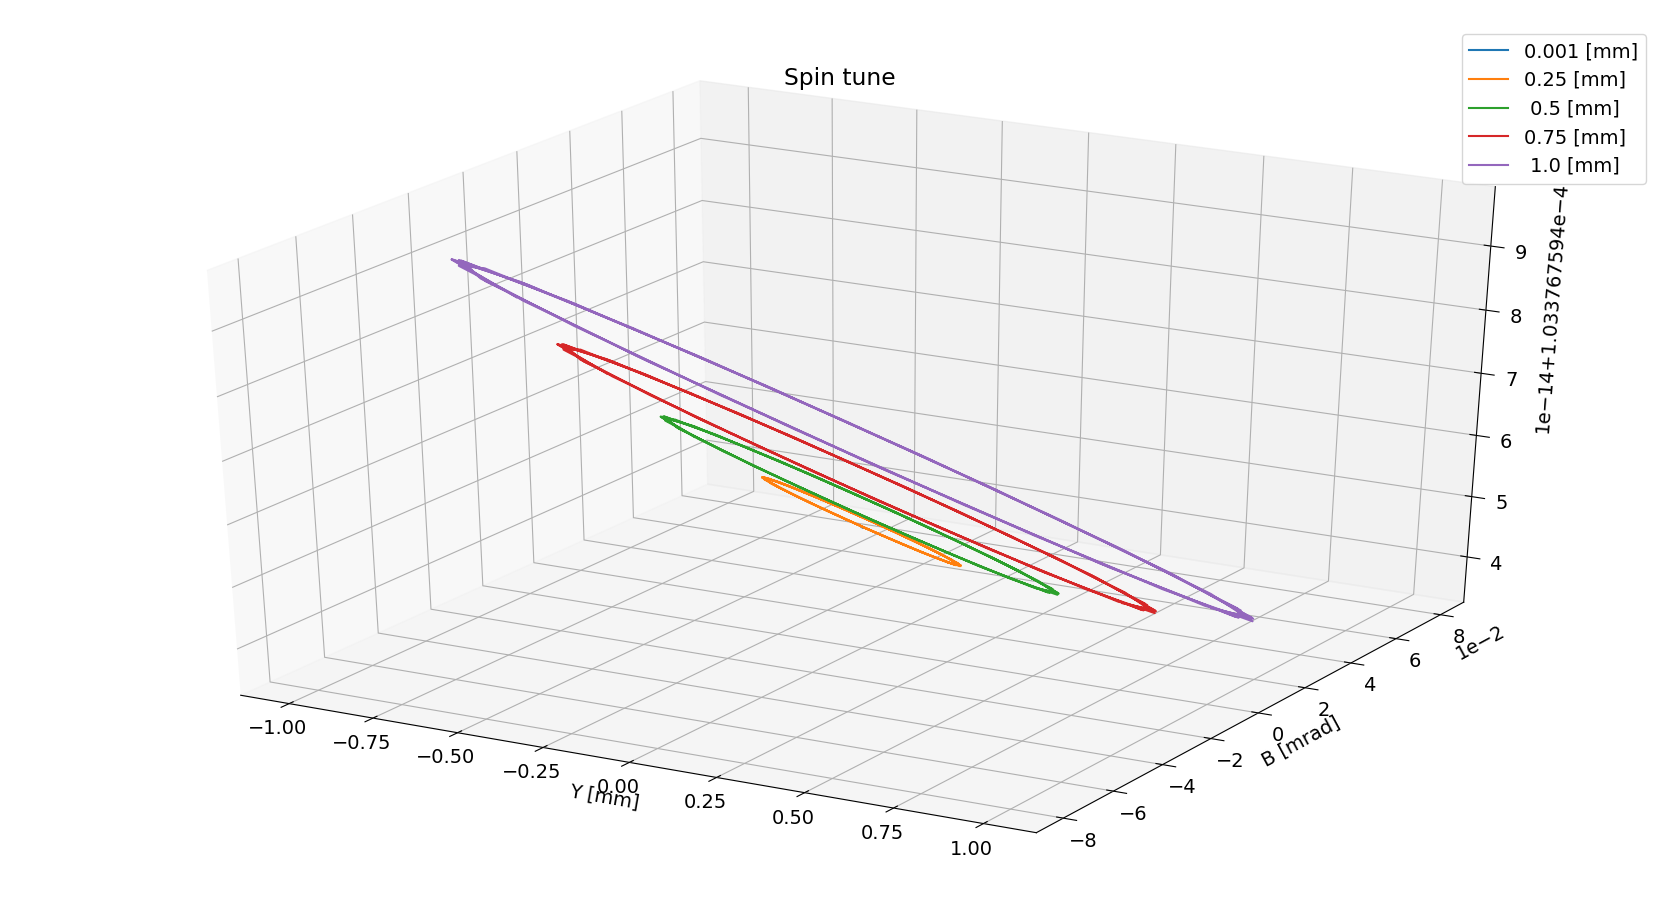
\includegraphics[width=\linewidth]{../img/IPAC19/ST_VS_YB_IMPERFECT_OPTIM}
%%     \caption{Spin tune.}
%%   \end{subfigure}
%%   \begin{subfigure}{\linewidth}\centering
%%     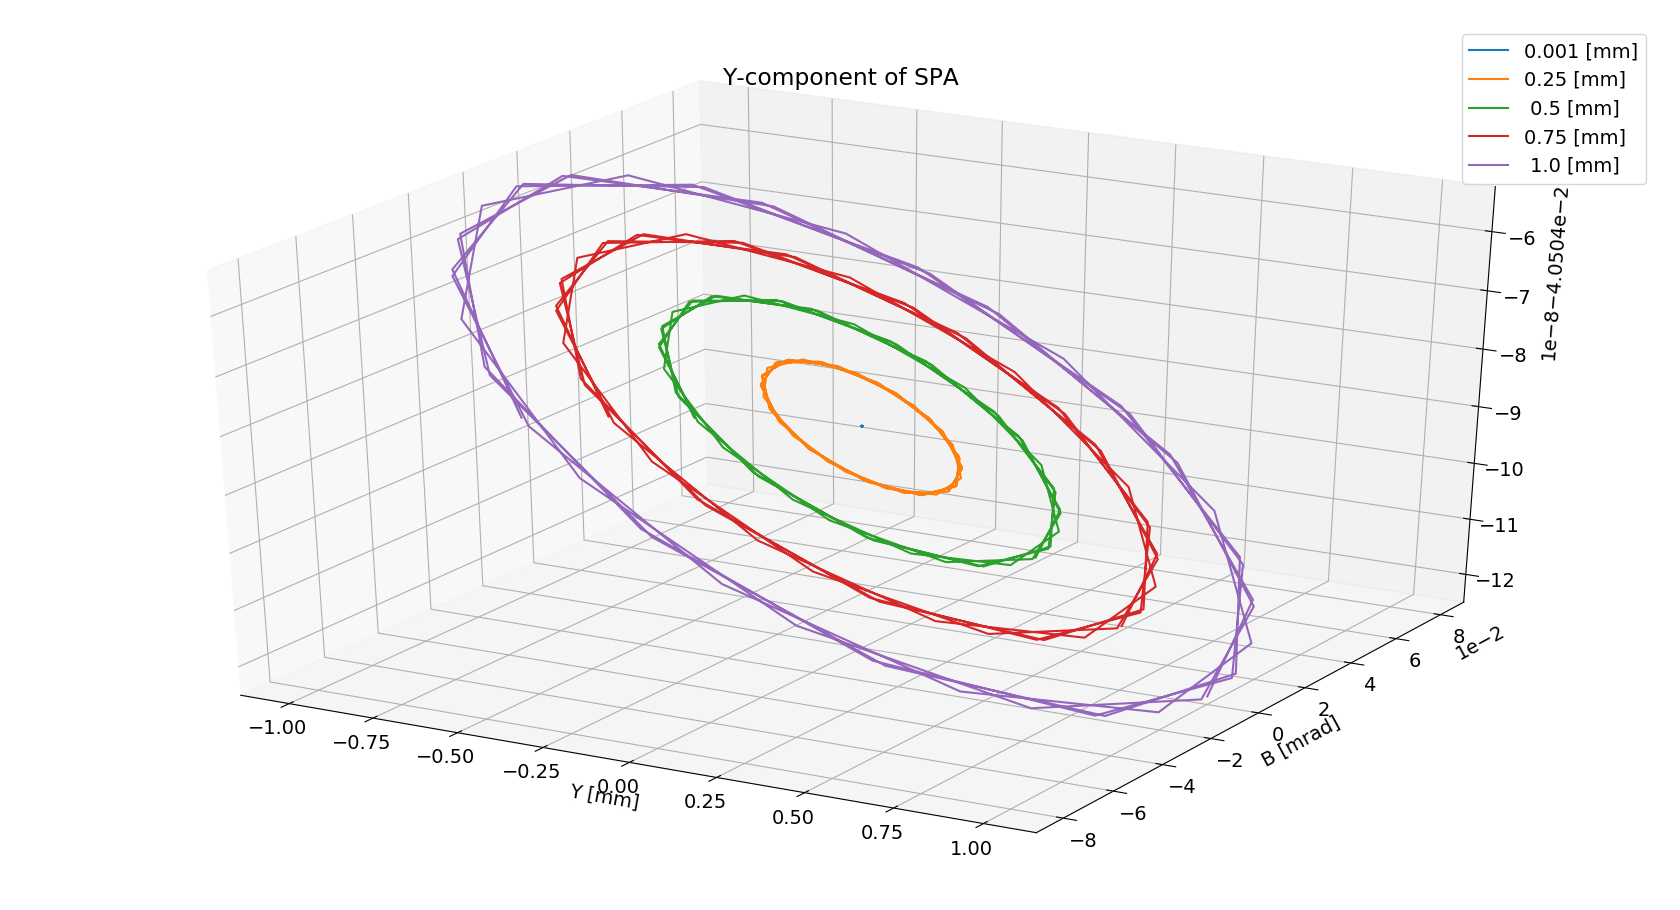
\includegraphics[width=\linewidth]{../img/IPAC19/NY_VS_YB_IMPERFECT_OPTIM}
%%     \caption{Vertical component of the invariant spin axis.}
%%   \end{subfigure}
%%   \caption{Spin tune and invariant spin axis computed on the particle phase space trajectories in a lattice
%%   optimizing spin decoherence caused by vertical plane betatron oscillations.\label{fig:3d_plots}}
%% \end{figure}

The three spin component time series were analyzed via residual functions
$\epsilon_1 = S_Y^{gen} - s_y^{idl}$ and $\epsilon_1 = S_Y^{trk} - s_y^{idl}$, as well as by fitting
model~\eqref{eq:fit_model} and comparing its goodness-of-fit.

\begin{figure}[h]
  \centering
  \begin{subfigure}{\linewidth}
    \centering
    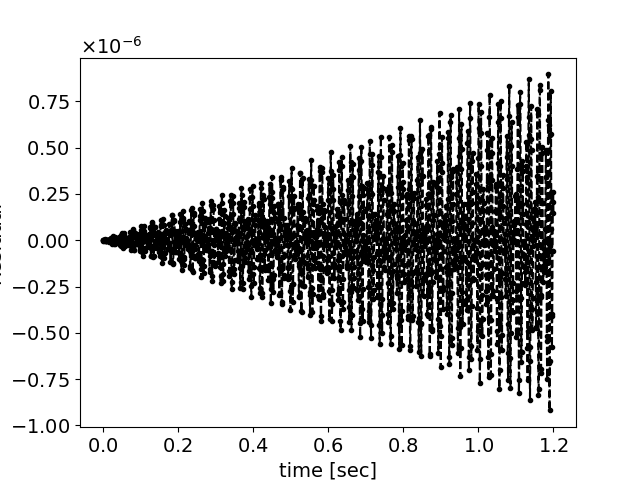
\includegraphics[width=\linewidth]{../img/IPAC19/GEN-IDL_RESIDUAL}
    \caption{$\epsilon_1 = s_y^{gen} - s_y^{idl}$ residual\label{fig:res:gens}}
  \end{subfigure}
  \begin{subfigure}{\linewidth}
    \centering
    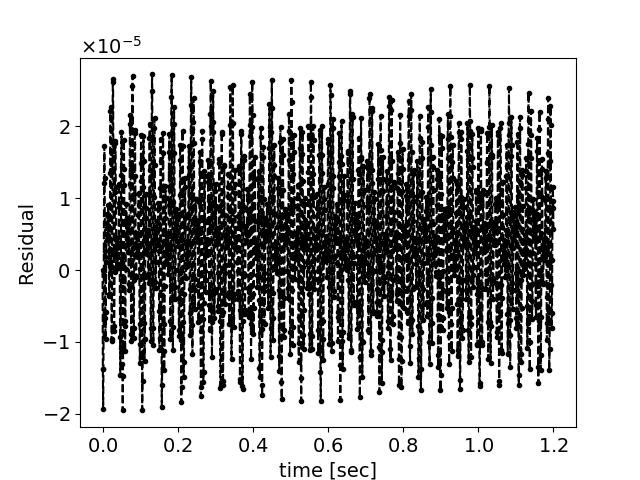
\includegraphics[width=\linewidth]{../img/IPAC19/TRK-IDL_RESIDUAL}
    \caption{$\epsilon_2 = s_y^{trk} - s_y^{idl}$ residual\label{fig:res:trkr}}
  \end{subfigure}
  \begin{subfigure}{\linewidth}
    \centering
    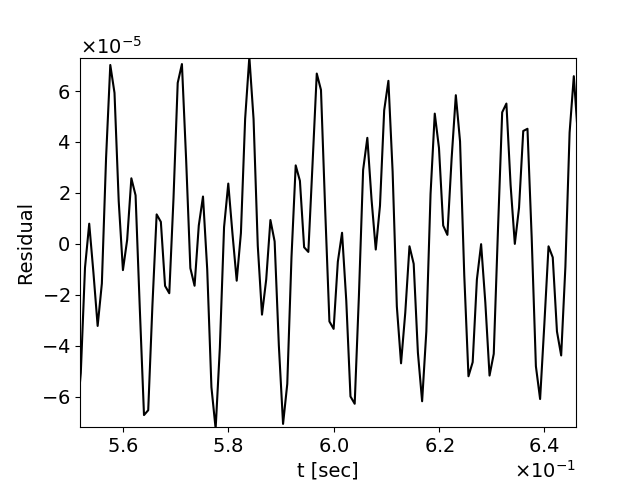
\includegraphics[width=\linewidth]{../img/IPAC19/TRK-IDL_RESIDUAL_section}
    \caption{Section of Figure~\ref{fig:res:trkr}\label{fig:tres:trkr_sec}}
  \end{subfigure}
    \caption{Time series' comparator residuals\label{fig:residuals}}
\end{figure}

The residuals $\epsilon_1$ and $\epsilon_2$ are plotted in Figure~\ref{fig:residuals}.
From Figure~\ref{fig:res:gens} one can observe that the generator series nearly approximates the ideal,
constant parameter sinusoid, whereas Figures~\ref{fig:res:trkr} and~\ref{fig:res:trkr_sec} indicate
that the $s_y^{trk}$-series performs oscillations relative to $s_y^{idl}$ with an amplitude
$\approx 10^{-4}$, and frequency 


\begin{table}[h]
  \caption{Parameter estimates table\label{tbl:param_estimates}}
  \begin{tabular}{r|rllr}
    \toprule
    Series & Par. & Value & St.Error & AIC \\
    \midrule
    \multirow{3}{*}{$s_y^{idl}$} & $\hat f$ & 74.452466549766214 & $6\cdot10^{-15}$ & \multirow{3}{*}{-86246} \\
    & $\hat a$ & 0.99841729771960 & $1\cdot10^{-14}$ & \\
    & $\hat\delta$ & 3.14159265358978 & $2\cdot 10^{-14}$ &\\
    \hline
    \multirow{3}{*}{$s_y^{gen}$} & $\hat f$ & 74.452466548 & $1\cdot 10^{-9}$ & \multirow{3}{*}{-49917} \\
    & $\hat a$ & 0.998417300 & $2\cdot 10^{-9}$ & \\
    & $\hat\delta$ & 3.1415926564 & $4\cdot 10^{-9}$ &\\
    \hline
    \multirow{3}{*}{$s_y^{trk}$} & $\hat f$ & 74.4524675 & $6\cdot 10^{-7}$ & \multirow{3}{*}{-30665} \\
    & $\hat a$ & 0.998418 & $1\cdot10^{-6}$ & \\
    & $\hat\delta$ & 3.141589 & $3\cdot 10^{-6}$ &\\
    \bottomrule
  \end{tabular}
\end{table}

\section{Conclusions}
The question of the influence of betatron motion on the EDM statistic in the FD method should be considered
in view of three circumstances:
\begin{enumerate}
\item The signal amplitude oscillations are small. They occur at the $10^{-4}$ level, whereas the expected
  polarization measurement error is on the order of percents. This means the superposition of this systematic
  error with the random measurement error will exhibit no statistically-significant systematicity.
\item The correllation coefficient between the amplitude and frequency estimates is not significant. The amplitude
  oscillations affect the $\hat a$-estimate foremost; their effect on the $\hat\w$-estimate is secondary, and is
  described by the correlation coefficient. Since it is less than 10\%, even if the oscillations happen to be
  strong enough to affect the amplitude estimate, their effect on the frequency estimate will be reduced by
  at least a factor of 10.
\item This systematic effect is controllable. And this point is the major advantage of the FD methodology.
  By applying an external Spin Wheel, the $\nbar$ oscillations can be continuously minimized
  as much as necessary, without changing the experiment pattern.
\end{enumerate}

\begin{thebibliography}{9}

\bibitem{Senichev:FDM}
  Y. Senichev, A. Aksentev, A. Ivanov, E. Valetov, ``Frequency domain method of the search for the deuteron electric dipole moment in a storage ring with imperfections.'' In review.

\bibitem{BNL:SREDM}
  M Bai et al., SREDM Collaboration website: \url{https://www.bnl.gov/edm/}

\bibitem{BNL:Deuteron2008}
  D. Anastassopoulos et at., (srEDM Collaboration), ``Search for a permanent electric dipole moment of the deuteron nucleus at the $10^{-29}~e\cdot cm$ level,'' proposal as submitted to the BNL PAC, April 2008.

\bibitem{Talman:ElectricRings}
  R. Talman, ``Prospects for Electric Dipole Moment Measurement Using Electrostatic Accelerators.'' August 2018.

\bibitem{Mane:SpinWheel}
  S Mane, ``A distillation of Koop's idea of the Spin Wheel.'' arXiv:1509.01167 [physics] \url{http://arxiv.org/abs/1509.01167}

\bibitem{Koop:SW}
  I. A. Koop. ``Asymmetric energy colliding ion beams in the EDM storage ring.'' Proc. of IPAC13 (2013). \url{http://accelconf.web.cern.ch/accelconf/ipac2013/papers/tupwo040.pdf}

\bibitem{COSY:SpinTuneMapping}
  A. Saleev et al., (JEDI Collaboration), ``Spin tune mapping as a novel tool to probe the spin dynamics in storage rings.'' Phys.Rev.Accel.Beams 20 (2017) no.7, 072801

\bibitem{Aksentev:DecohIPAC19}
  A Aksentev, Y Senichev, ``Spin decoherence in the Frequency Domain Method for the search of a particle EDM.'' Proc. of IPAC19 (2019).

\bibitem{Senichev:Lattices}
  Y. Senichev, S. Andrianov, S. Chekmenev, M. Berz, E.Valetov. ``Investigation of Lattice for Deuteron EDM Ring.''
  Proc. of ICAP15 (2015). \url{http://accelconf.web.cern.ch/AccelConf/ICAP2015/papers/modbc4.pdf}

\bibitem{COSYINF:Website}
  M. Berz, K. Makino, COSY Infinity website: \url{cosyinfinity.org}

\bibitem{COSYINF:BeamPhysMan}
  M. Berz, K. Makino. COSY INFINITY 10.0 Beam Physics Manual.
  
%% \bibitem{Senichev:IPAC13}
%%   Y. Senichev, R. Maier, D. Zyuzin, N. Kulabukhova, (JEDI Collaboration), ``Spin tune decoherence effects in electro- and magnetostatic structures.'' Proc. of IPAC13 (2013).

\end{thebibliography} 
\end{document}
